% Template for Cogsci submission with R Markdown

% Stuff changed from original Markdown PLOS Template
\documentclass[10pt, letterpaper]{article}

\usepackage{cogsci}
\usepackage{pslatex}
\usepackage{float}
\usepackage{caption}

% amsmath package, useful for mathematical formulas
\usepackage{amsmath}

% amssymb package, useful for mathematical symbols
\usepackage{amssymb}

% hyperref package, useful for hyperlinks
\usepackage{hyperref}

% graphicx package, useful for including eps and pdf graphics
% include graphics with the command \includegraphics
\usepackage{graphicx}

% Sweave(-like)
\usepackage{fancyvrb}
\DefineVerbatimEnvironment{Sinput}{Verbatim}{fontshape=sl}
\DefineVerbatimEnvironment{Soutput}{Verbatim}{}
\DefineVerbatimEnvironment{Scode}{Verbatim}{fontshape=sl}
\newenvironment{Schunk}{}{}
\DefineVerbatimEnvironment{Code}{Verbatim}{}
\DefineVerbatimEnvironment{CodeInput}{Verbatim}{fontshape=sl}
\DefineVerbatimEnvironment{CodeOutput}{Verbatim}{}
\newenvironment{CodeChunk}{}{}

% cite package, to clean up citations in the main text. Do not remove.
\usepackage{apacite}

% KM added 1/4/18 to allow control of blind submission


\usepackage{color}

% Use doublespacing - comment out for single spacing
%\usepackage{setspace}
%\doublespacing


% % Text layout
% \topmargin 0.0cm
% \oddsidemargin 0.5cm
% \evensidemargin 0.5cm
% \textwidth 16cm
% \textheight 21cm

\title{Combinatorial Capacity of English Negation in Child Language}


\author{{\large \bf Morton Ann Gernsbacher (MAG@Macc.Wisc.Edu)} \\ Department of Psychology, 1202 W. Johnson Street \\ Madison, WI 53706 USA \AND {\large \bf Masoud Jasbi (jasbi@ucdavis.edu)} \\ Department of Linguistics, 469 Kerr Hall, One Shields Avenue \\ Davis, CA 95 USA}


\begin{document}

\maketitle

\begin{abstract}
Negation is very important for langauge and thought. How does it develop
in the language of children? There has been many guessses like
rejection, non-existence, denail, etc. but it has been hard to assess
because these concepts are vaguge. Here we assess the combinatorial
capacity of early negation in children's productions, and use words
negation combines with as a proxy for early concepts expressed by it. We
show some important stuff.

\textbf{Keywords:}
negation; combinatorial capacity; corpus anlysis.
\end{abstract}

\hypertarget{introduction}{%
\section{Introduction}\label{introduction}}

Negation is an abstract concept, lexicalized in all previously studied
human languages, and crucial to everyday communication. It can help a
coffee shop divide its menu into ``coffee'' and ``not coffee'' sections,
with the ``not coffee'' section bringing together diverse items that
otherwise cannot be labeled. It can help us regulate others' actions in
a sign like ``no mask, no entry''. It can also communicate our deepest
wants and dislikes. But how does this crucial abstract concept emerge in
humans? Does language play a role in its emergence or does language
simply adopt it for communication?

There has been several influential hypotheses on the conceptual origin
of negation.

In this paper, we address the same issues with a slightly different
approach. We start with the widely accepted assumption that negation is
a higher order operator or function, operating on lower level concepts.
The question we ask is: what type of concepts does linguistic negation
operate on in early child language? Do we find negation starting in a
limited conceptual domain and then expanding to others? Or do we find it
operating across different conceptual domains as early as we can attest
it?

Darwin (1998) thought that negation has roots in the expression of human
emotions and desires. He hypothesized that the earliest manifestation of
negation and affirmation in infants is when they refuse food from
parents, by withdrawing their heads laterally, or when they accept the
food, by inclining their heads forward. He suggested that head shaking
and nodding as common gestures for negation and affirmation have
developed from this early habit. Considering early functions of negative
morphemes like \emph{no}, many researchers proposed that children use
them to ``reject'' or ``refuse'' (Bloom, 1970; Choi, 1988; Pea, 1978).
For example, they may say ``no'' when asked ``do you want juice?'', say
``not want it'', or say ``don't like it''. Pea (1978) proposed that this
function of negation is the first to emerge in children.

Motor control: prohibition (do not spill milk), inability (I cannot zip
it)

Bloom (1970) suggested that the first function of negation in children's
speech is to express non-existence. Relates to children's development of
object permanence.

Perceptual: non-existence (no juice, no more milk, no fish in the
bathroom, I do not have underpants), failure, Locatives (no in there,
daddy was not on the phone), non-events (the dog not barking)

A third possible domain and path to the acquisition of negation is
language itself. Word learning places its own constraints on the
conceptual space. One possibility is that negation develops, and is
aided by the act of labeling and categorizing objects and actions for
linguistic communication. This function would manifest istelf in
labeling acts with nominal predicates such as ``this is not a bunny'',
``not red'', or ``this isn't a reptile''.

There has been no proposal for negation originating in the child's
understanding of her own or other's epistemic states. In fact, most
development theory of mind accounts assume that this ability emerges
later in children. However, many corpus instances of negation modify
mental state verbs such as \emph{know}, \emph{think}, and
\emph{remember} (e.g.~``I not know''). Therefore, we also report the
prevalence and emergence of such cases.

Caveat on production vs comprehension.

Emphasize that we are focusing on the utterance level in this study

Quantitative validations of previous work

New grouping

\hypertarget{experiments}{%
\section{Experiments}\label{experiments}}

\hypertarget{data-and-preprocessing}{%
\subsection{Data and preprocessing}\label{data-and-preprocessing}}

For developmental data of child language in English, we turned to the
CHILDES database (MacWhinney, 2000), which provides child-parent
conversational
interactions.\footnote{Code and data are in quarantine at https://somewhereonearth.}.
We focused on speech produced by children with typical development
within the age range of 12 - 72 months. As this study focuses on
negation constructions at the utterance-level, we extracted individual
utterances with any of the three negation markers to be investigated in
this study: \emph{no}, \emph{not} and \emph{n't}. Utterances with only
one lexical token (e.g.~\emph{no !}) were not considered as here we aim
to address particularly the question of what negation markers could
\emph{combine} with. In addition, cases where the negation markers only
serve as a discourse marker (e.g.~\emph{no I like this one} /\emph{no no
no Mommy}) were excluded as well. Preprocessing led to a data set of
365,260 utterances with negation structures from a total of 811 children
across 56 corpora.

Figure @ref(fig:speaker\_stats)

\begin{CodeChunk}
\begin{figure}[H]

{\centering 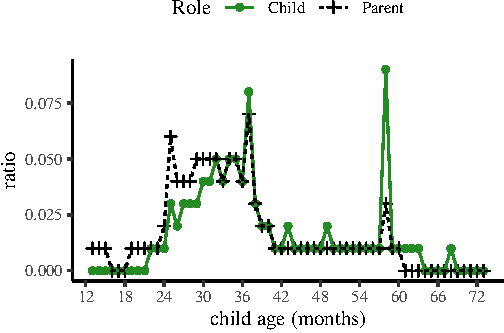
\includegraphics{figs/speaker_stats-1} 

}

\caption[Distribution of the number of utterances with negative morphemes in child and parent speech]{Distribution of the number of utterances with negative morphemes in child and parent speech.}\label{fig:speaker_stats}
\end{figure}
\end{CodeChunk}

\hypertarget{negation-functions}{%
\subsection{Negation functions}\label{negation-functions}}

In this section, we describe in details our automatic extraction of
syntactic structures that have distinct negation functions and express
different types of negative concepts. The current English data from
CHILDES contains morphosyntactic information (Sagae, Davis, Lavie,
MacWhinney, \& Wintner, 2010) such as part-of-speech (POS) information
as well as grammatical or syntactic dependency
relations.\footnote{Besides using the provided POS and syntactic dependency information in CHILDES, we also experimented with the state-of-the-art parser from Stanza [@qi-etal-2020-stanza], an open-source natural language processing library. There were no worth noting differences in the analyses for the negation constructions.}
We take advantage of information as such when identifying our
constructions of interest. Since most of the available annotations were
obtained via the existing tools in CHILDES, in order to further
alleviate potential errors induced from the automatic process, an
utterance with a negative morpheme(s) was only considered when the
negative morpheme has either a POS of \emph{neg} or \emph{qn}, the
latter of which was mainly for cases with \emph{no} as a quantifier.
Furthermore, the syntactic functions and relations of the negative
morphemes should not be enumeration (\emph{no no no}), communicators or
discourse markers.

After extracting all instances with negative morphemes, the
developmental trajectory of each construction type as described in the
previous section was analyzed. While the matter of interest here is
child speech, we also compared patterns in child production to those in
parent speech as references at the corresponding age of the child. Then
we combined the development of all construction types for analysis as a
whole.

\hypertarget{rejection}{%
\subsubsection{Rejection}\label{rejection}}

Under the broader context of expressing emotion (Darwin, 1998), we
focused particularly on utterances that function as rejections.
Specifically, we examined cases where the lemma form of the head verb of
the phrase is either \emph{like} or \emph{want}, and the head verb is
modified by one of the three negative morphemes. Each of the utterances
either takes a subject or has no subject at all. And the existence of a
subject was determined via searching for a word in the utterance that
has the \emph{SUBJ} dependency relation with the head verb.

Additionally, other than expressions that the speaker used to describe
their own emotion (e.g.~(1)) or their (in)ability to do so (e.g.~(2)),
we also included cases that express rhetorical inquiries of emotions
from one interlocutor addressed to another (e.g.~(3)) as well as
instances where the speaker is describing the emotion of somebody else
(e.g.~(4)). Overall our data extraction resulted in a total of 21,034
utterances (Child: 9,608; Parent: 11,426).

~ (1) \emph{I no like sea} / \emph{don't wanna go}

~ (2) \emph{I can't like that}

~ (3) \emph{don't you wanna try it}

~ (4) \emph{Sarah doesn't like that either}

To compare the patterns between child and parent speech, for the
function of rejection, as well as for all other functions that negation
serve (see below), we measured the following four metrics as indexes of
developmental characteristics if applicable. These metrics were applied
to child and parent utterances respectively. The first one is the
relative ratio of each of the three negative morphemes overall. For
instance, given the 9,608 from child speech that serve as rejections,
there are 8,531 cases with the negative morpheme \emph{no}; then the
ratio of these utterances was calculated as 8,531 / 9,608 = 0.41.

The second one is the relative ratio of negative morphemes within
different head verbs (e.g.~\emph{like} vs.~\emph{want} for rejection).
For example, again with child speech that express rejections, utterances
where the negative morphemes modify the head verb \emph{like} occur for
3,268 times; then the ratio of these cases was computed as 3,268 / 9,608
= 0.16.

The third one is the relative ratio of the negative utterances at
different ages of the child. For instance, for rejection, at the age of
36 months, the total number of instances with the negative morphemes in
child speech is 888; then their ratio was calculated as 888 / 9,608 =
0.04.

The last one is the amount of variability in the production of the
specific function across the age span of the child, which was measured
with entropy (Cover \& Thomas, 1991) For example, after computing the
relative ratio (\emph{P(x\_i)}) of the negative utterances at a number
of \(N\) ages of the child for the specific function, the production
variability is calculated as the equation below.

\[
H(X) = -\sum_{i=1}^N P(x_i)log_2P(x_i)               
\]

In both child and parent speech, when articulating emotion with either
of the two head verbs \emph{like} and \emph{want}, the most frequently
used negative morpheme is \emph{n't} combined with an auxiliary verb.
Comparing the two different head verbs, overall the negative morphemes
co-occur with \emph{want} more frequently. With that being said, the
amount of variability in both child and parent production is similar, a
pattern that holds for both head verbs (Child \emph{like}: 0.12; Child
\emph{want} 0.12; Parent \emph{like}: 0.12; Parent \emph{want}: 0.12).

On the other hand, when looking at the developmental trajectory, as
presented in Figure @ref\{fig:emotion\}, children's usage of negative
morphemes is comparable regardless of the particular head verb. In
general, children start applying the negative morphemes for the function
of rejection more regularly around the age of 22 months. Within the
context of the corpus data that we analyzed, their usage of these
morphemes is the most frequent during the age range of 25 - 36 months,
then gradually decreases as they age.

\begin{CodeChunk}
\begin{figure}[H]

{\centering 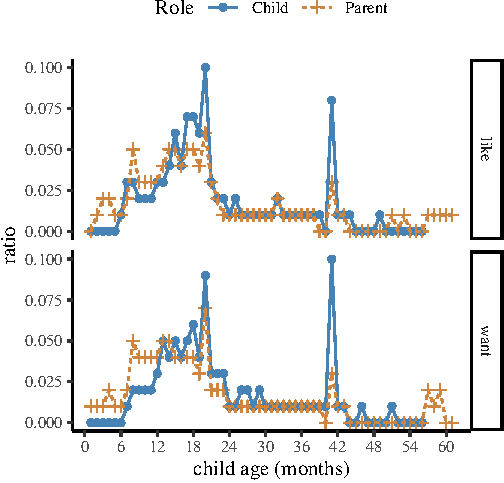
\includegraphics{figs/emotion-1} 

}

\caption[Rejection]{Rejection}\label{fig:emotion}
\end{figure}
\end{CodeChunk}

\hypertarget{epistemic-state}{%
\subsubsection{Epistemic state}\label{epistemic-state}}

With regards to the broader domain of theory of mind, we attended to
cases where the negative morphemes modify epistemic state. In
particular, we focused on utterances that articulate the concept of
unknowing (e.g.~(5)) or uncertainty (e.g.~(6)). The cases that were
subject to analyses here included either \emph{know}, \emph{remember} or
\emph{think} as the head verb, modified by the negative morphemes or the
combination of negation with auxiliaries. By these search criteria,
instances where the speaker inquires about or describes the negative
epistemic position of another speaker (e.g.~(7)) were also selected.
This led to a subset of 32,793 utterances in total (Child: 10,389;
Parent: 22,404).

~ (5) \emph{I not know} / \emph{I didn't remember}

~ (6) \emph{I don't think so}

~ (7) \emph{don't you remember} / \emph{She doesn't know this}

In both child and parent speech, the most frequently used negative
morpheme that modifies epistemic state is \emph{n't}, a pattern that is
consistent across the three different head verbs. And the negative
morphemes tend to co-occur more often in cases that describe the state
of unknowing, which is indicated mainly by the verb \emph{know}. Based
on results from Figure @ref\{fig:epistemic\}, the production of
\emph{know} for expressions of epistemic state starts earlier in
comparison to \emph{remember} and \emph{think}. On the other hand, the
production variability for each of the head verb (\textasciitilde0.12)
is comparable to each other regardless of the particular speaker.
Overall, children began to apply the negative morphemes to articulate
this function in a more regular fashion around the age of 25 months.

\begin{CodeChunk}
\begin{figure}[H]

{\centering 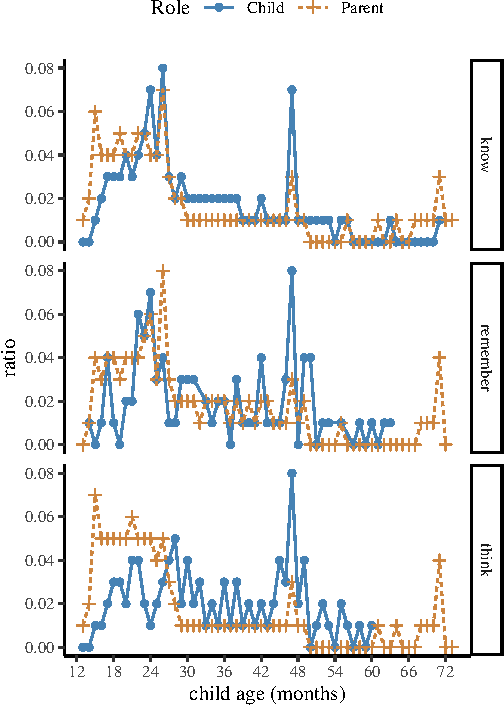
\includegraphics{figs/epistemic-1} 

}

\caption[Epistemic]{Epistemic}\label{fig:epistemic}
\end{figure}
\end{CodeChunk}

\hypertarget{prohibition}{%
\subsubsection{Prohibition}\label{prohibition}}

For utterances that articulate the function of prohibition, we focused
on cases where the negative morphemes are combined with the auxiliary
verb \emph{do} (\emph{do}, \emph{does}, \emph{did}) and the auxiliary
does not take any subject (e.g.~(8)). In certain cases the negative
morphemes and the auxiliary together modifies a head verb. For instances
as such, in order to not overlap with the function of rejection,
epistemic state, non-existence and possession (see below), our search
excluded cases where the head verb has any of the following lemma forms:
\emph{like}, \emph{want}, \emph{know}, \emph{think}, \emph{remember},
\emph{have}. This resulted in a total of 21,197 utterances (Child:
6,140; Parent: 15,057).

After applying our metrics, overall the most frequently used negative
morpheme is \emph{n't} when articulating prohibition. The amount of
production variability for this function is comparable in both child and
parent speech, with an approximate value of 0.12. The developmental
trajectory of using the negative morphemes to serve this function
(Figure @ref{[}fig:prohibition{]}) is comparable to that of the previous
ones, where children started more regular usage of negative morphemes
around the age of 23 months.

~ (8) \emph{don't blame Charlotte} / \emph{don't}

\begin{CodeChunk}
\begin{figure}[H]

{\centering 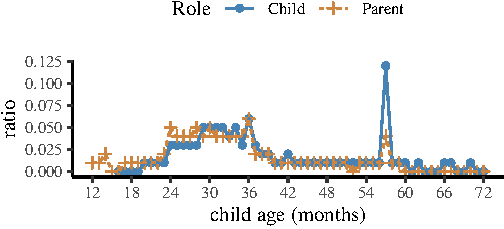
\includegraphics{figs/prohibition-1} 

}

\caption[Prohibition]{Prohibition}\label{fig:prohibition}
\end{figure}
\end{CodeChunk}

\hypertarget{inability}{%
\subsubsection{Inability}\label{inability}}

With regards to the function of inability, we analyzed instances where
the negative morphemes co-occur with the auxiliary \emph{can}
(\emph{can} and \emph{could}; e.g.~(9)). Again, for instances with a
head verb modified by the negatiive morphemes and the auxiliary, we
filtered out cases where the head verbs are the focus for other
functions, the same way as our analyses for the function of prohibition
analyzed above. Cases that do not have a subject (\emph{can't play}) or
do not contain a subject other than I (\emph{you can't do that}) could
yield ambiguous readings without taking a larger discourse context into
account; they could be a rhetorical question or also express the concept
of prohibition. Therefore to avoid potential ambiguity, we excluded
instances as such. In other words, when searching for utterances that
articulate inability, we restricted our analyses only to cases with a
subject \emph{I}. This led to a subset of 9,150 utterances (Child:
5,410; Parent: 3,740).

~ (9) \emph{I can't see} / \emph{I can't}

Comparing child and parent production, the negative morpheme that is
used most frequently is also \emph{n't}. As shown in Figure
@ref\{fig:inaibility\} The developmental trajectory of this function is
similar to that for prohibition, and the negative morphemes are applied
more regularly starting around the age of 23 months. The amount of
production variability in both child and parent speech is approximately
0.12.

\begin{CodeChunk}
\begin{figure}[H]

{\centering 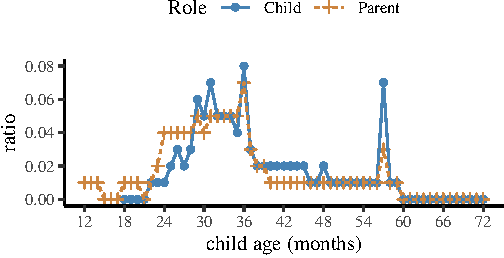
\includegraphics{figs/inability-1} 

}

\caption[Inability]{Inability}\label{fig:inability}
\end{figure}
\end{CodeChunk}

\hypertarget{language-learning-via-labeling}{%
\subsubsection{Language learning via
labeling}\label{language-learning-via-labeling}}

For the function of language learning, particularly labeling, we
concentrated on cases where negative morphemes are adopted to indicate
the identity (e.g.~(10)), and/or characteristics (e.g.~(11)) of a
predicative nominal. In addition, we also included instances where the
negative morphemes are used to modify a predicative adjective
(e.g.~(12)). Following these criteria, utterances where the negative
morpheme is modifying a nominal or adjectival predicate of a copula verb
were extracted. None of the utterances contained expletives (\emph{there
is no book}). The existence of a predicate was identified with the help
of POS information and dependency relation. The POS of the predicate has
to be either noun (\emph{n}) or adjective (\emph{adj}), and its
dependency relation with the copula has to be \emph{PRED}. This resulted
in a total of 20,329 utterances (Child: 4,793; Parent: 15,536).

~ (10) \emph{that's not a farmer}

~ (11) \emph{I'm not a heavy baby Mum}

~ (12) \emph{It's no good}

Comparing the three negative morphemes, the most frequently used is
\emph{not} regardless of the specific speaker, and the amount of
production variability is comparable (\textasciitilde0.12) between child
and parent speehc. Based on results from Figure @ref\{fig:learning\},
the developmental trajectory of using the negative morphemes in the
domain of language learning is comparable to previous domains. Children
started using the negative morphemes for the function of labeling
nominal objects more frequently around the age of 24 months; yet their
usage gradually decreases around the age of 36 months.

\begin{CodeChunk}
\begin{figure}[H]

{\centering 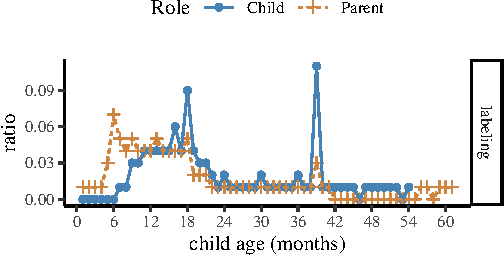
\includegraphics{figs/learning-1} 

}

\caption[Language learning via labeling]{Language learning via labeling}\label{fig:learning}
\end{figure}
\end{CodeChunk}

\hypertarget{non-existence}{%
\subsubsection{Non-existence}\label{non-existence}}

The utterances to be analyzed here are cases combined with negative
morphemes to express the function of non-existence. To do that, we
extracted utterances that either have expletives marked by \emph{there}
(e.g.~(13)), or cases where the negative morphemes are modifying a
nominal (i.e.~its syntactic head based on the CHILDES annotation is a
nominal; e.g.~(14)). With utterances such as (14) in particular, in
order to not confuse with the function of labeling, we did not include
any cases where the syntactic head of the negative morphemes is a
predicate of a copula verb (e.g.~\emph{this is not candy}). This led to
a total of 34,672 utterances (Child: 16,866; Parent: 17,806).

~ (13) \emph{there's no water}

~ (14) \emph{no (more) candy} / \emph{not your mouth}

In both child and parent speech, the most frequently occurred negative
morphemes to indicate non-existence is \emph{no}. The amount of
production variability approximates 0.12 regardless of the specific
speaker. Again for comparison of child and parent speech, we calculated
the relative ratio of (i) each of the three negative morphemes overall;
(ii) usage of negative morphemes with the two different communicative
functions; (iii) utterances expression motor control with the three
negative morphemes at different ages of the child. Overall the most
frequently used negative morpheme is \emph{n't} when applied in the
domain of motor control. Comparing the two communicative functions, the
negative morphemes tend to co-occur more often when expressing
inability.

As shown in Figure @ref\{fig:existence\}, children began increasing
their use of the negative morphemes to express non-existence around the
age of 22 months, whereas the frequency of applying these negative
morphemes started to become less regular around the age of 36 months.

\begin{CodeChunk}
\begin{figure}[H]

{\centering 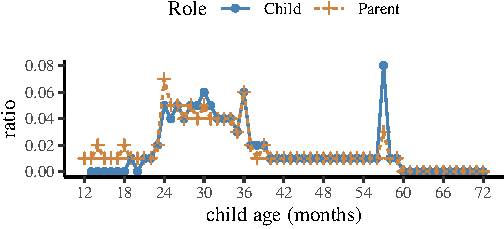
\includegraphics{figs/existence-1} 

}

\caption[Non-existence]{Non-existence}\label{fig:existence}
\end{figure}
\end{CodeChunk}

\hypertarget{possession}{%
\subsubsection{Possession}\label{possession}}

The last function that we investigated includes utterances that are
combined with negative morphemes to denote possession. Specifically, we
selected cases where the negative morphemes are modifying a possessive
pronoun (e.g.~(15)), as well as instances where the negative morphemes
are combined with auxiliary verbs to modify a head verb with the lemma
form \emph{have} (e.g.~(16)). Again similarly to our search for
utterances that express non-existence, we excluded cases in which the
syntactic head of the negative morphemes is a predicate of a copula verb
(e.g.~\emph{this is not mine}). As a result, the total of utterances
that were subjected to analysis for this function is 9,265 (Child:
2,899; Parent: 6,366). The developmental trajectory for this function,
as shown in Figure @ref{[}fig:possession{]}, is comparable to that for
the function of non-existence.

~ (15) \emph{not mine}

~ (16) \emph{I don't have it}

\begin{CodeChunk}
\begin{figure}[H]

{\centering 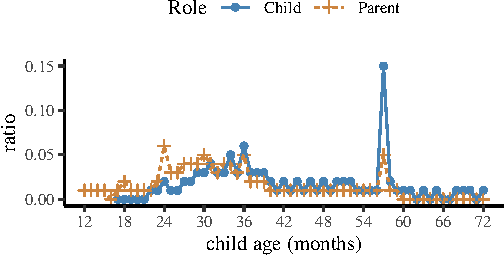
\includegraphics{figs/possession-1} 

}

\caption[Possession]{Possession}\label{fig:possession}
\end{figure}
\end{CodeChunk}

\hypertarget{an-overall-look-at-all-functions}{%
\subsubsection{An overall look at all
functions}\label{an-overall-look-at-all-functions}}

\begin{figure*}[h]
\begin{CodeChunk}


\begin{center}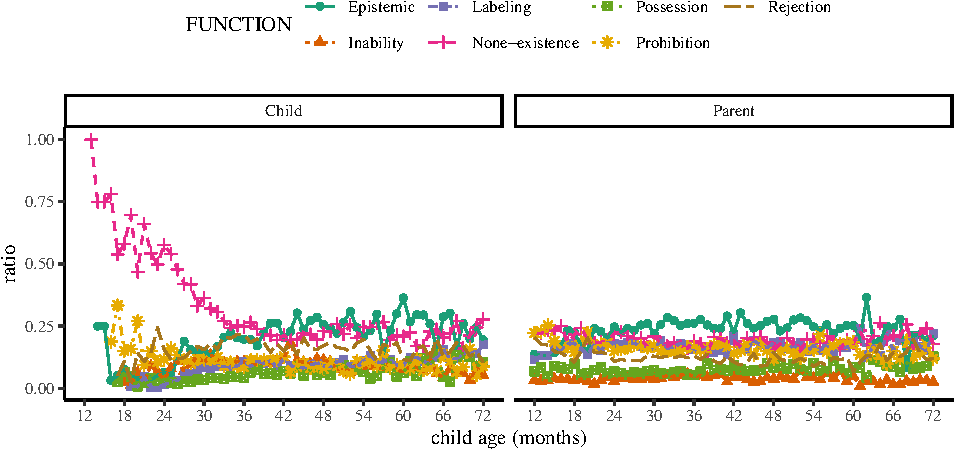
\includegraphics{figs/all-1} \end{center}

\end{CodeChunk}
\caption[This image spans both columns]{All functions.}\label{fig:all}
\end{figure*}

\begin{figure*}[h]
\begin{CodeChunk}


\begin{center}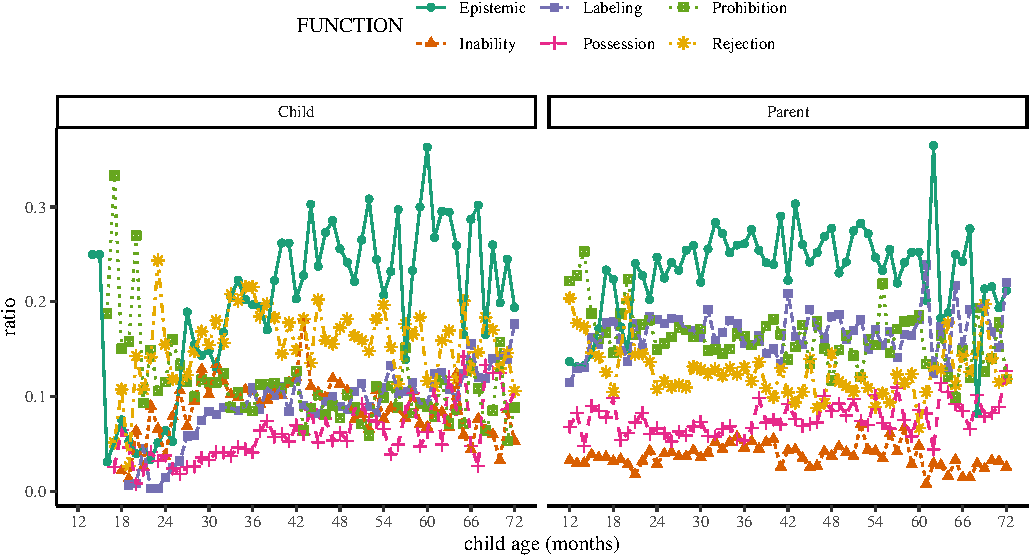
\includegraphics{figs/exclude-1} \end{center}

\end{CodeChunk}
\caption[This image spans both columns]{All functions except for None-existence.}\label{fig:exclude}
\end{figure*}

In this section, we combined all negative utterances analyzed above to
examine how the production trajectory of each function develops \emph{in
relation to} the other functions. Therefore, the index of developmental
characteristics for each function was measured as the relative ratio of
the number of utterances within the particular function given a specific
age of the child. For example, the total number of utterances with
negative morphemes in child speech at the age of 66 months is 253, in
which cases that express rejection have a frequency of 32. Then the
relative ratio of the rejection function at this age is measured as 32 /
253 = 0.13.

As presented in Figure@ref\{fig:all\}, child speech with negative
morphemes bears considerable amount of similarity with parent speech in
terms of the overall production patterns. The most frequently applied
function is non-existence, while the functions with relatively smaller
number of occurrences include possession and inability.

With that being said, there are a number of observant differences
between child and parent utterances with respects to the amount of
production variability. In both child and parent production, the
function that has the highest amount of variability is non-existence
(Child: ; Parent: ).

With that being said,

the overall production pattern as well as the pattern for each
individual function.

On the other hand, in comparison, the differences in production
variability are more observant with the functions of prohibition (Child:
; Parent: ) and labeling (Child: ; Parent: ).

\hypertarget{discussion}{%
\section{Discussion}\label{discussion}}

For future work, we would like to extend our current study in three
respects. First, while here the analyses were restricted to only
utterances with negative morphemes, we plan to also investigate the
positive counterpart structures of these cases (e.g.~\emph{I don't know}
vs.~\emph{I know}). This would allow us to see how the production
trajectory of the negative morphemes develops within the broader context
of particular syntactic constructions (Goldberg, 1995). Secondly,
besides looking at the utterances produced by all children or parents,
we intend to narrow our focus to the developmental trajectory of
individual child, the data for which ideally contains production from a
wider age range (e.g.~12 - 72 months.), This would allow us to further
investigate individual differences in the development of negation.
Lastly, our experiments thus far have concentrated on the utterance
level, therefore cases where negations are used as discourse markers
were excluded. However, discourse markers indeed have important roles in
the communication between children and parents, where the negative
morphemes could also be indicating the functions that have been analyzed
above (e.g.~Parent: \emph{do you want some bread?}; Child: \emph{no no
no}). More thorough examinations of discourse-level instances as such
would paint a more clear picture about the production of negation.

\hypertarget{references}{%
\section{References}\label{references}}

\setlength{\parindent}{-0.1in} 
\setlength{\leftskip}{0.125in}

\noindent

\hypertarget{refs}{}
\leavevmode\hypertarget{ref-bloom1970language}{}%
Bloom, L. M. (1970). \emph{Language development: Form and function in
emerging grammars} (PhD thesis). Columbia University.

\leavevmode\hypertarget{ref-choi1988semantic}{}%
Choi, S. (1988). The semantic development of negation: A
cross-linguistic longitudinal study. \emph{Journal of Child Language},
\emph{15}(3), 517--531.

\leavevmode\hypertarget{ref-cover_elements_1991}{}%
Cover, T. M., \& Thomas, J. A. (1991). \emph{Elements of information
theory}. New York: Wiley.

\leavevmode\hypertarget{ref-darwin1872expression}{}%
Darwin, C. (1998). \emph{The expression of the emotions in man and
animals}. John Murray.

\leavevmode\hypertarget{ref-goldberg1995constructions}{}%
Goldberg, A. E. (1995). \emph{Constructions: A construction grammar
approach to argument structure}. University of Chicago Press.

\leavevmode\hypertarget{ref-macwhinney2000childes}{}%
MacWhinney, B. (2000). \emph{The childes project: Tools for analyzing
talk. Transcription format and programs} (Vol. 1). Psychology Press.

\leavevmode\hypertarget{ref-pea1978}{}%
Pea, R. (1978). \emph{The development of negation in early child
language} (PhD thesis). University of Oxford.

\leavevmode\hypertarget{ref-sagae2010morphosyntactic}{}%
Sagae, K., Davis, E., Lavie, A., MacWhinney, B., \& Wintner, S. (2010).
Morphosyntactic annotation of childes transcripts. \emph{Journal of
Child Language}, \emph{37}(3), 705--729.

\bibliographystyle{apacite}


\end{document}
